\documentclass{standalone}
\usepackage{tikz}
\usepackage{nono}
\usepackage{siunitx}

\begin{document}
%\usepgfplotslibrary{colormaps} 
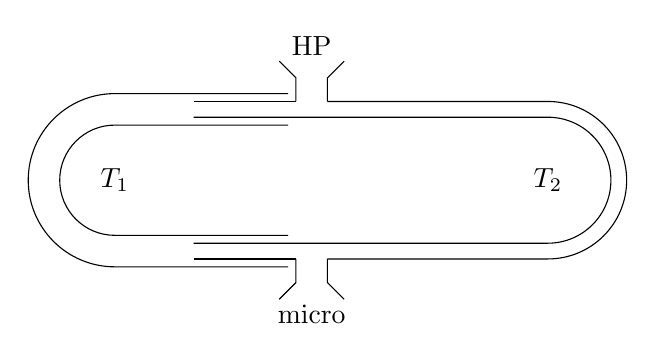
\begin{tikzpicture} 
  \draw (0.2, 1) -- (3, 1) arc (90:-90:1) -- (0.2, -1);
  \draw (-1.5, 1) -- (-0.2, 1) (-0.2, -1) -- (-1.5, -1);
  \draw (-1.5, 0.8) -- (3, 0.8) arc (90:-90:0.8) -- (-1.5, -0.8);

  \draw (-0.3, 1.1) -- (-2.5, 1.1) arc (90:270:1.1) -- (-0.3, -1.1);
  \draw (-0.3, 0.7) -- (-2.5, 0.7) arc (90:270:0.7) -- (-0.3, -0.7);

  \draw (0.2, 1) -- ++(0, 0.3) -- ++(45:0.3);
  \draw (-0.2, 1) -- ++(0, 0.3) -- ++(135:0.3);
  \draw (0, 1.7) node{HP}; 

  \draw (0.2, -1) -- ++(0, -0.3) -- ++(-45:0.3);
  \draw (-0.2, -1) -- ++(0, -0.3) -- ++(-135:0.3);
  \draw (0, -1.7) node{micro}; 

  \draw (-2.5, 0) node{$T_1$};
  \draw (3, 0) node{$T_2$};
\end{tikzpicture}
\end{document}
